\documentclass[hyperref={bookmarks=true}]{beamer}
   \title[Network analysis with Cytoscape]{Network analysis with Cytoscape}
   \author[Group 1]{presented by Kai, Stefan \& Stephan}
   \date{02/08/2012}
   \institute[lecture on systems bioinformatics]{in lecture on systems bioinformatics}

   \usepackage{amsmath}
   \usepackage{subfigure}
   \usepackage{booktabs}
   \usepackage{color}
   \usepackage{stmaryrd}
   \usepackage{movie15}
   \usepackage[utf8]{inputenc}
   \usepackage[T1]{fontenc}
   \usepackage{ae,aecompl}
   \usepackage{listings}
   \usepackage{courier}
   \lstset{
         basicstyle=\tiny,
 %        basicstyle=\footnotesize\ttfamily, % Standardschrift
         numbers=left,               % Ort der Zeilennummern
         numberstyle=\tiny,          % Stil der Zeilennummern
         stepnumber=1,               % Abstand zwischen den Zeilennummern
         numbersep=5pt,              % Abstand der Nummern zum Text
         tabsize=1,                  % Groesse von Tabs
         extendedchars=true,         %
         breaklines=true,            % Zeilen werden Umgebrochen
         keywordstyle=\color{blue},
         frame=b,         
         stringstyle=\color{green}\ttfamily, % Farbe der String
         showspaces=false,           % Leerzeichen anzeigen ?
         showtabs=false,             % Tabs anzeigen ?
         xleftmargin=17pt,
         framexleftmargin=17pt,
         framexrightmargin=5pt,
         framexbottommargin=4pt,
         commentstyle=\color{red},
         showstringspaces=false      % Leerzeichen in Strings anzeigen ?        
   }
   \lstloadlanguages{Java} 

   \usepackage{caption}
   \DeclareCaptionFont{white}{\color{white}}
   \DeclareCaptionFormat{listing}{\colorbox[cmyk]{0.43, 0.35, 0.35,0.01}{\parbox{\textwidth}{\hspace{15pt}#1#2#3}}}
   \captionsetup[lstlisting]{format=listing,labelfont=white,textfont=white, singlelinecheck=false, margin=0pt, font={bf,footnotesize}}

   \setlength{\heavyrulewidth}{0.10em}
   \setlength{\lightrulewidth}{0.03em}
   \numberwithin{equation}{subsection}

   \usetheme{Boadilla}
   \usecolortheme{whale}
   \mode<presentation>
   \hypersetup
   {
      pdfauthor={Stephan Matthias Grein},
      pdftitle={VL Systembiologie},
      pdfsubject={Netzwerke, topologische Charakteristika, Zentralitäten},
      bookmarksopen=true,
      bookmarksopenlevel=3,
      bookmarksnumbered,
      pageanchor,
      plainpages=false
   }

   \newtheorem*{remark}{Remark}
   \newtheorem*{aims}{Aims}
   \newcommand{\myspace}{\vspace{0.2em}}
   \renewcommand*\thesubfigure{(\alph{subfigure})}
   \renewcommand*\figurename{Fig. \thefigure}

\begin{document}
   \begin{frame}
 \titlepage
\end{frame}
\begin{frame}
 \frametitle{Outline}
 \tableofcontents
\end{frame}
\AtBeginSection[]
{
  \begin{frame}[plain]{Outline}
    \tableofcontents[currentsection,currentsubsection]
  \end{frame}
}

   \section{Introduction}
\begin{frame}{Introduction I}
\dots why should we care about glycolysis and gluconeogeneses
\end{frame}

\begin{frame}{Introduction}
	\begin{itemize}
		\item using the tool CellDesigner to build a glycolysis/gluconeogenese network,
		\item import it into the tool Cytoscape,
		\item analyse the imported network and
		\item implement missing centralities and indices by coding some plugins
	\end{itemize}
\end{frame}

\begin{frame}{Glycolysis/Gluconeogenese}
	\begin{itemize}
		\item catabolic linear pathway of glycolysis deals with the breakdown and extraction of energy from glucose
		\item the reverse anabolic process - gluconeogenesis - is equally important
		\item gluconeogenesis helps to keep blood glucose levels within critical limits
		\item these processes provide many points for regulation
	\end{itemize}
\end{frame}

\begin{frame}{Glycolysis}
	\begin{figure}[htbp]
	   \centering
	   \includegraphics[width=0.6\textwidth]{inc/img/circle}
	   \caption{Glycolysis vs. Gluconeogenese}
	   \label{fig:circle}
	\end{figure}
\end{frame}

\begin{frame}{Glycolysis}
	\begin{figure}[htbp]
	   \centering
	   \includegraphics[width=0.6\textwidth]{inc/img/equation}
	   \caption{Glycolysis vs. Gluconeogenese}
	   \label{fig:circle}
	\end{figure}
\end{frame}

\begin{frame}{Glycolysis and Disease}
	\begin{itemize}
		\item Genetic disease - mutations are generally rare due to importance of the metabolic pathway
		\item Cancer - typically tumor cells have glycolytic rates that are up to 200 times higher
		\item Other disease - disfunctioning glycolysis or glucose metabolism has been associated with some other diseases
	\end{itemize}
\end{frame}

\begin{frame}{Glycolysis and Cancer}
	\begin{itemize}
		\item Ubiquitous gene overexpression appears to be restricted to glycolysis, in conclusion, Glycolysis is indeed special.
		\item this may also be of some interest for therapy, increased Glucose consumption can be observed with clinical tumour imaging 
		\item Gene expression patterns in general can be modified by external factors such as drugs or components of nutrition
		\item one may envision substances that modify expression of glycolysis genes as complementary to conventional cancer therapies
	\end{itemize}
\end{frame}

\begin{frame}
	\begin{itemize}
		\item
	\end{itemize}
\end{frame}

\begin{frame}
	\begin{itemize}
		\item
	\end{itemize}
\end{frame}

\begin{frame}{Literature}
	\begin{itemize}
		\item R. A. Gatenby and R. J. Gillies, Why do cancers have high aerobic glycolysis?, Nature Review Cance, Vol. 4, p. 891-899, November 2004.
		\item B. Altenberga and K.O. Greulich, Genes of glycolysis are ubiquitously overexpressed in 24 cancer classes, Genomics Vol. 84, p. 1014-1020, September 2004.
	\end{itemize}
\end{frame}

\begin{frame}{Cell Designer}
	\begin{itemize}
		\item tried to model a glycolysis network
		\item tool very user unfriendly
		\item export into a format for cytoscape resulted in "strange" networks
		\item this task was skipped
	\end{itemize}
\end{frame}

\begin{frame}{Cytoscape}
	\begin{itemize}
		\item provides many useful plugins 
		\item plugin KGMLReader used to import KEGG Glycolysis network
		\item modified the network to make it user readable
		\item 
	\end{itemize}
\end{frame}


\begin{frame}{Introduction II}
\dots basic setup of our two networks ... how we modelled them and what did not work (CellDesigner) ...
\end{frame}



   \section{Code}
\begin{frame}{Plugin for calculation of Katz's Index}
\begin{definition}[Katz's Index]
Let $A$ denote the adjacency matrix of a \textbf{directed} or \textbf{undirected} graph with dim($A$) $=$ $n \times n$ and let $\alpha$ denote a non-negative damping factor.
\begin{equation}
I_{Katz}(i) = \sum_{k=1,..,\infty} \sum_{j=1,..n} \alpha(A^k)_{ji}
\end{equation}
$\Leftrightarrow$
\begin{equation}\label{eq:2}
I_{Katz} = ((\mathbb{I}_m - \alpha A^T)^ {-1} - \mathbb{I}_m) \mathbb{I}_v
\end{equation}
\end{definition}
For calculations we used Eq. \ref{eq:2} and considered two distinct cases:
\begin{enumerate}
\item $\alpha$ small $\Rightarrow$ emulation of degree centrality
\item $\alpha \in$ $]0,\frac{1}{|\lambda_{max}|}]$ $\Rightarrow$ influence of pathes weighted
\end{enumerate}
\end{frame}
\begin{frame}{Plugin for calculation of Katz's Index - $\alpha$ $\equiv$ 0.1}
\lstinputlisting[firstnumber=1, language=Java, label=KatzPlugin,caption=Necessary import statements]{inc/source/plugin1/Lst1.java}
\end{frame}
\begin{frame}{Plugin for calculation of Katz's Index - $\alpha$ $\equiv$ 0.1}
\lstinputlisting[firstnumber=16, language=Java, label=KatzPlugin,caption=Basic class definition]{inc/source/plugin1/Lst2.java}
\end{frame}
\begin{frame}{Plugin for calculation of Katz's Index - $\alpha$ $\equiv$ 0.1}
\lstinputlisting[firstnumber=38, language=Java, label=KatzPlugin,caption=Run method (I)]{inc/source/plugin1/Lst3.java}
\end{frame}
\begin{frame}{Plugin for calculation of Katz's Index - $\alpha$ $\equiv$ 0.1}
\lstinputlisting[firstnumber=57, language=Java, label=KatzPlugin,caption=Run method (II)]{inc/source/plugin1/Lst4.java}
\end{frame}
\begin{frame}{Plugin for calculation of Katz's Index - $\alpha \equiv \frac{1}{|\lambda_{max}|}$}
\lstinputlisting[firstnumber=57, language=Java, label=KatzPlugin,caption=Run method (II)]{inc/source/plugin2/Lst5.java}
\end{frame}

\begin{frame}{Plugin for calculation of Randic's Index}
\begin{definition}[Randics's Index]
Let $v(i)$ denote the \#neighbors of vertex $v$ with index $i$ and $N$ \#nodes.
\begin{equation}
I_{Randic} = \sum_{i=0}^{N-1} \frac{1}{\sqrt{v(i)}}
\end{equation}
\end{definition}
\begin{exampleblock}{Cave}
Randic's Index works only for \textbf{undirected} and \textbf{connected} graphs.
\end{exampleblock}
\pause
\begin{block}{Application}
Currently there is no known application of Randic's Index for the analysis of biological networks.
\end{block}
\end{frame}
\begin{frame}{Plugin for calculation of Randic's Index}
\lstinputlisting[firstnumber=1, language=Java, label=RandicPlugin,caption=Necessary import statements]{inc/source/plugin3/Lst6.java}
\end{frame}
\begin{frame}{Plugin for calculation of Randic's Index}
\lstinputlisting[firstnumber=16, language=Java, label=RandicPlugin,caption=Basic class definition]{inc/source/plugin3/Lst7.java}
\end{frame}
\begin{frame}{Plugin for calculation of Randic's Index}
\lstinputlisting[firstnumber=38, language=Java, label=RandicPlugin,caption=Run method]{inc/source/plugin3/Lst8.java}
\end{frame}

   \section{Results}
%-------------------------------------------------
\begin{frame}{Results - Centralities}
	\begin{itemize}
		\item determine the relative importance of a vertex within a graph
		\item centraltity concepts were first developed in social network analysis
		\begin{description}
			\item[-->] e.g. how influential a person is within a social network
		\end{description}
	\end{itemize}
	
	\begin{definition}[Four measures of centrality]
		\begin{enumerate}
			\item degree centrality
			\item eccentricity centrality			
			\item closeness centrality
			\item betweeness centrality
		\end{enumerate}
	\end{definition}
\end{frame}
%-------------------------------------------------
\begin{frame}{Results - Degree Centrality}
	\begin{definition}[Degree Centrality]
		$C_{deg}(v) = \{e|e \in E\; and\; v \in e\}$
	\end{definition}
	\begin{itemize}
		\item counts the number of edges attached to a vertex
		\item a local centrality measure
		\begin{description}
			\item[-->] only direct neighborhood considered 
		\end{description}
		\item directed graphs:
		\begin{description}
			\item[-->] indegree (interpreted as "popularity")
			\item[-->] outdegree (interpreted as "gregariousness")
		\end{description}
	\end{itemize}
\end{frame}
%-------------------------------------------------
\begin{frame}{Results - Degree Centrality}
\begin{figure}
	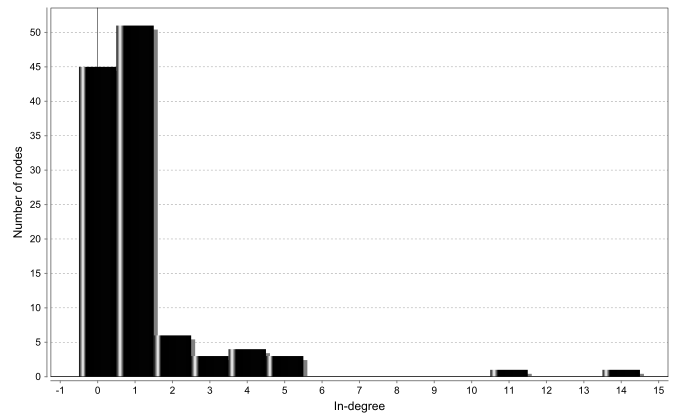
\includegraphics[scale=0.4]{inc/img/Glyco1/InDegreeDistr.png}
%\subfigure[Glyco1]{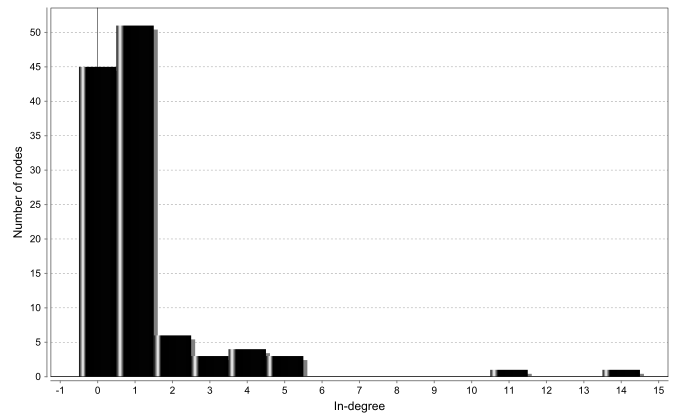
\includegraphics[scale=0.25]{inc/img/Glyco1/InDegreeDistr.png}}\hfill
%\subfigure[Glyco2]{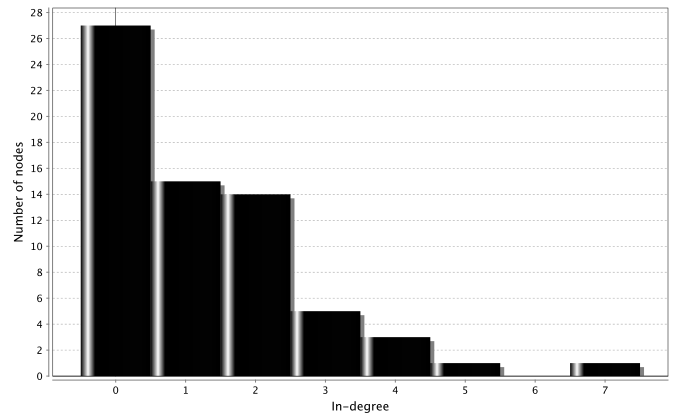
\includegraphics[scale=0.25]{inc/img/Glyco2/InDegree.png}}
\caption{Indegree Centrality}
\end{figure}
\end{frame}
%-------------------------------------------------
\begin{frame}{Results - Degree Centrality}
\begin{figure}
	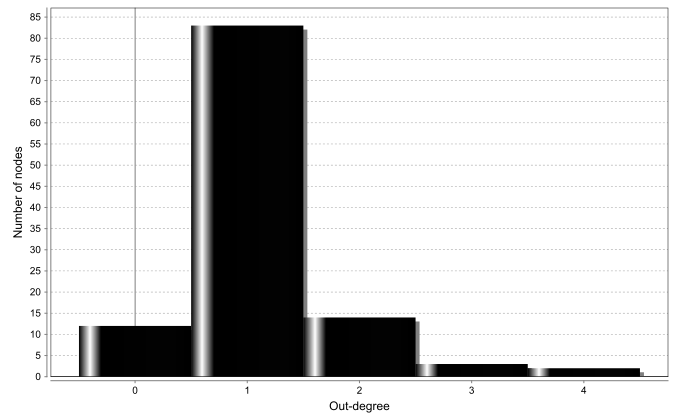
\includegraphics[scale=0.4]{inc/img/Glyco1/OutDegreeDistr.png}
%\subfigure[Glyco1]{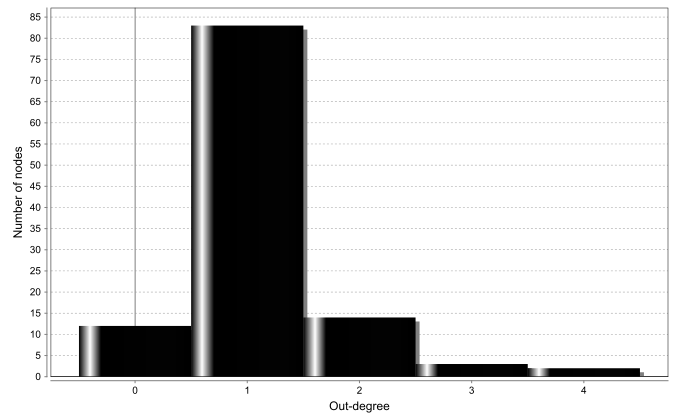
\includegraphics[scale=0.25]{inc/img/Glyco1/OutDegreeDistr.png}}\hfill
%\subfigure[Glyco2]{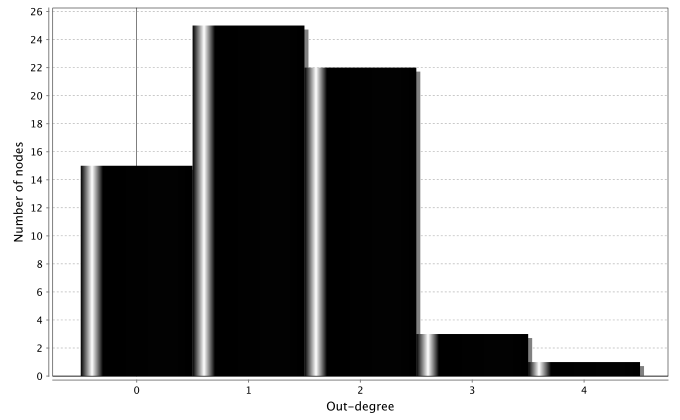
\includegraphics[scale=0.25]{inc/img/Glyco2/OutDegree.png}}
\caption{Outdegree Centrality}
\end{figure}
\end{frame}
%-------------------------------------------------
\begin{frame}{Results - Eccentricity Centrality}
	\begin{definition}[Eccentricity Centrality]
		$C_{ecc}(s) = \frac{1}{max\{d_{st}|t\in V\}}$
	\end{definition}
	\begin{itemize}
		\item determine the maximum distance between every two vertices
		\item central vertices get low values
		\item centralities require high centrality values
		\begin{description}
			\item[-->] reciprocal is used as centrality value
		\end{description}
		\item only for CONNECTED networks
	\end{itemize}
\end{frame}
%-------------------------------------------------
\begin{frame}{Results - Eccentricity Centrality}
	\begin{figure}
		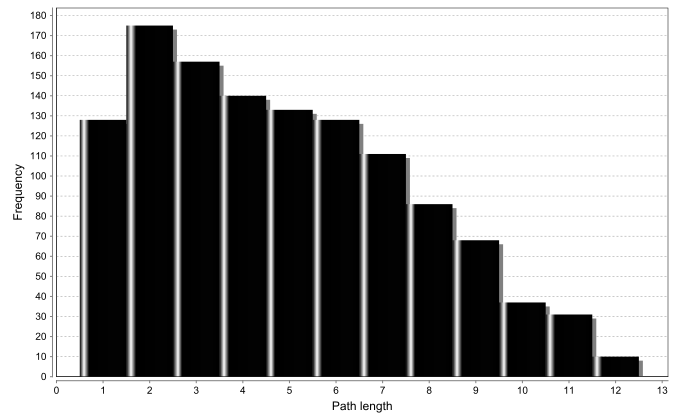
\includegraphics[scale=0.4]{inc/img/Glyco1/ShortPathLengthDistr.png}
	%\subfigure[Glyco1]{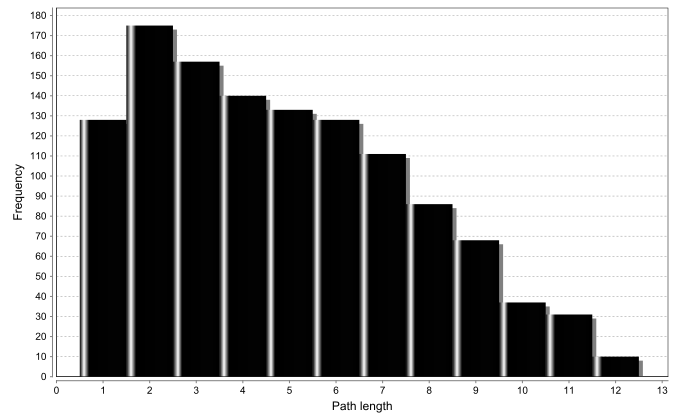
\includegraphics[scale=0.25]{inc/img/Glyco1/ShortPathLengthDistr.png}}\hfill
	%\subfigure[Glyco2]{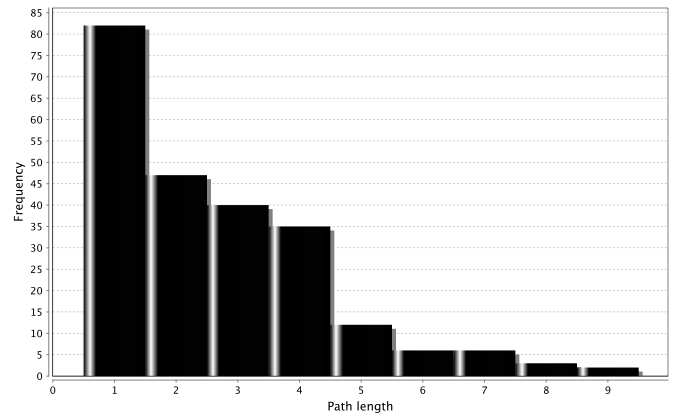
\includegraphics[scale=0.25]{inc/img/Glyco2/ShortestPathLengthDistr.png}}
	\caption{Eccentricity Centrality}
	\end{figure}
\end{frame}
%-------------------------------------------------
\begin{frame}{Results - Closeness Centrality}
	\begin{definition}[Closeness Centrality]
		$C_{clo}(s) = \frac{1}{\sum\limits_{t\in V} d_{st}}$
	\end{definition}
	\begin{itemize}
		\item $C_{clo}$ of a vertex s is the sum of shortest path form s to all other vertices  
		\item degree of interaction in the network
		\item the closer a point is to all the rest, the more effective and independent he can reach them
	\end{itemize}
\end{frame}
%-------------------------------------------------
\begin{frame}{Results - Closeness Centrality}
	\begin{figure}
		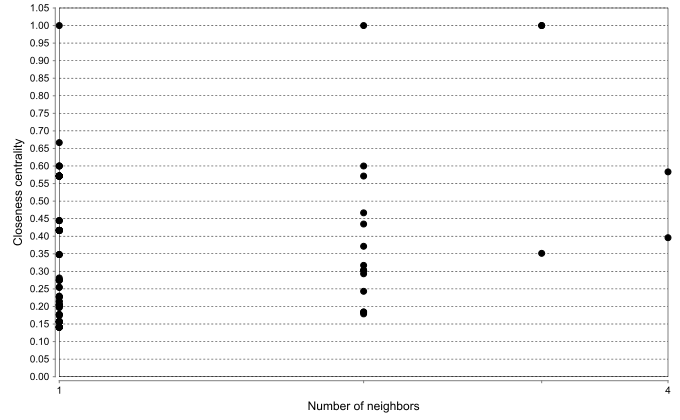
\includegraphics[scale=0.4]{inc/img/Glyco1/ClosenessCentr.png}
	%\subfigure[Glyco1]{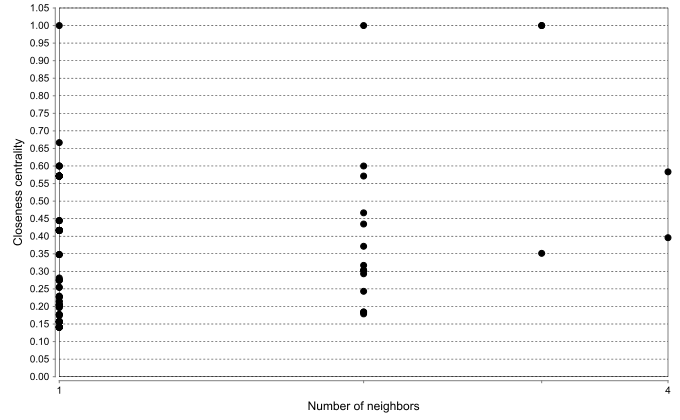
\includegraphics[scale=0.25]{inc/img/Glyco1/ClosenessCentr.png}}\hfill
	%\subfigure[Glyco2]{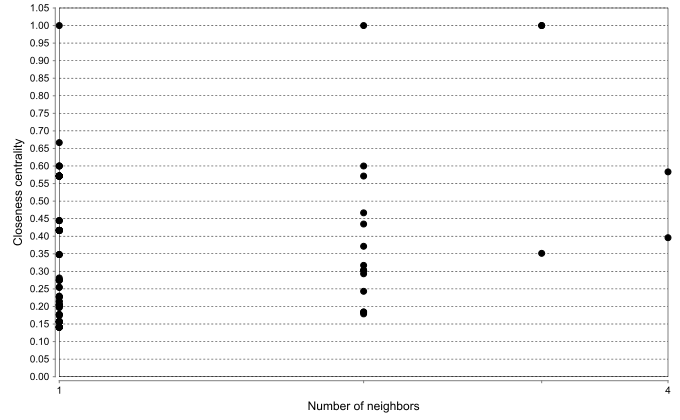
\includegraphics[scale=0.25]{inc/img/Glyco1/ClosenessCentr.png}} %TODO hier noch für Glyco 2 einbinden
	\caption{Closeness Centrality}
	\end{figure}
\end{frame}
%-------------------------------------------------
\begin{frame}{Results - Betweenness Centrality}
	\begin{definition}[Betweenness Centrality]
		$C_{spb}(v)=\sum\limits_{s \in V\; and\; s \neq v} \sum\limits_{t \in V\; and\; s \neq v} \delta_{st}(v)$
	\end{definition}
	\begin{itemize}
		\item center of attention: indirect relationships 
		\begin{description}
			\item[-->] Control of interaction
		\end{description}
		\item v is the more powerful the more shortest paths between other vertices it can interrupt
	\end{itemize}
\end{frame}
%-------------------------------------------------
\begin{frame}{Results - Betweenness Centrality}
	\begin{figure}
		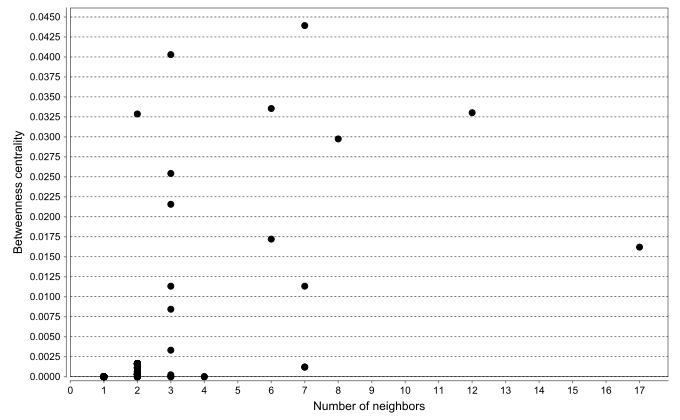
\includegraphics[scale=0.4]{inc/img/Glyco1/BetweennessCentr.png}
	%\subfigure[Glyco1]{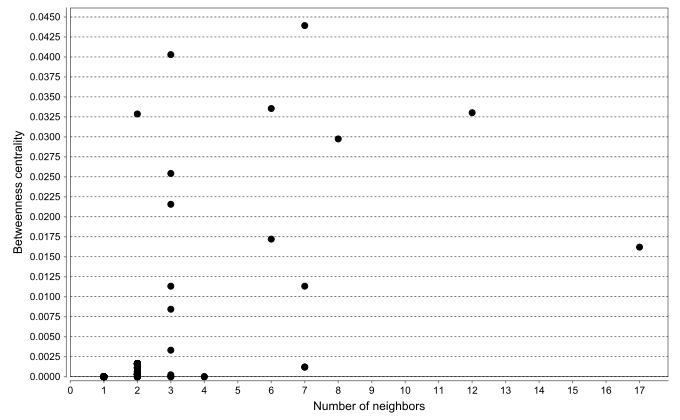
\includegraphics[scale=0.25]{inc/img/Glyco1/BetweennessCentr.png}}\hfill
	%\subfigure[Glyco2]{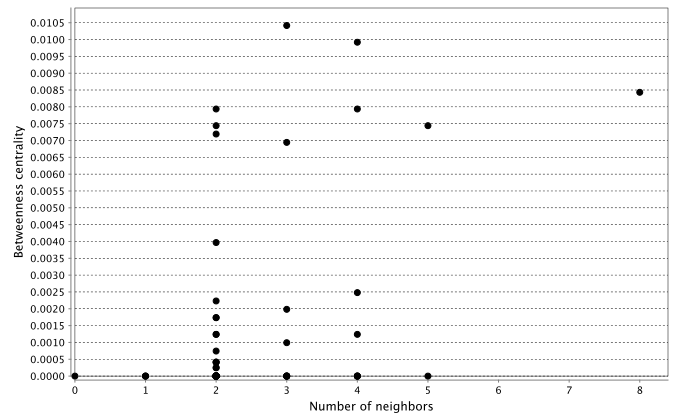
\includegraphics[scale=0.25]{inc/img/Glyco2/BetweennessCentr.png}}
	\caption{Closeness Centrality}
	\end{figure}
\end{frame}
%-------------------------------------------------
\begin{frame}{Results - Conclusion}
	\begin{itemize}
		\item the analysis tools are not very helpful
		\begin{description}
			\item[-->] cannot see which vertex has which centrality
			\item[-->] only give a statistical overview of the whole network
		\end{description}
		\item \textbf{but} you can select a vertex in the network window and get an overview of all centralities from the selected vertex
	\end{itemize}
\end{frame}
%-------------------------------------------------
\begin{frame}{Results - Betweenness Centrality}
	\begin{figure}
		\includegraphics[scale=0.35]{inc/img/Glyco1/Vertex_Centricities.PNG}
	%\subfigure[Glyco1]{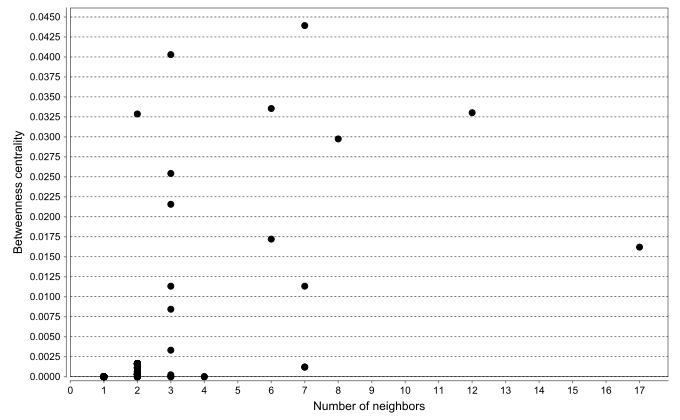
\includegraphics[scale=0.25]{inc/img/Glyco1/BetweennessCentr.png}}\hfill
	%\subfigure[Glyco2]{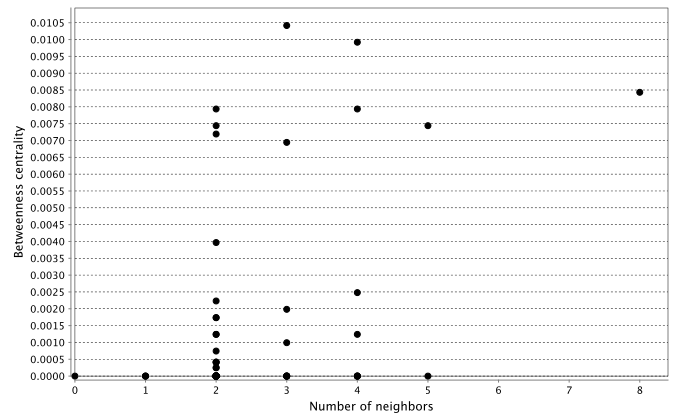
\includegraphics[scale=0.25]{inc/img/Glyco2/BetweennessCentr.png}}
	\caption{Centrality Overview}
	\end{figure}
\end{frame}
   \section{Resources}
\begin{frame}{Resources}
\begin{block}{Git repository}
git://gitorious.org/cytoscape-plugins/cytoscape-plugins.git
\end{block}
\end{frame}

\end{document}
